\documentclass[12pt,letterpaper,oneside,reqno]{amsart}
\usepackage{amsfonts}
\usepackage{amsmath}
\usepackage{amssymb}
\usepackage{amsthm}
\usepackage{float}
\usepackage{mathrsfs}
\usepackage{colonequals}
\usepackage[font=small,labelfont=bf]{caption}
\usepackage[left=1in,right=1in,bottom=1in,top=1in]{geometry}
\usepackage[pdfpagelabels,hyperindex,colorlinks=true,linkcolor=blue,urlcolor=magenta,citecolor=green]{hyperref}
\usepackage{graphicx}
\linespread{1.7}
\emergencystretch=1em
\usepackage{array}
\usepackage{etoolbox}
\apptocmd{\sloppy}{\hbadness 10000\relax}{}{}
\raggedbottom

% rascal numbers
\newcommand \rascalNumber [3] {\binom{#1}{#2}_{#3}}
\newcommand \north[0] {\mathit{North}}
\newcommand \south[0] {\mathit{South}}
\newcommand \west[0] {\mathit{West}}
\newcommand \east[0] {\mathit{East}}

% 1-q pascal notation

\newcommand{\genstirlingI}[3]{%
    \genfrac{[}{]}{0pt}{#1}{#2}{#3}%
}
\newcommand{\genstirlingII}[3]{%
    \genfrac{\{}{\}}{0pt}{#1}{#2}{#3}%
}
\newcommand{\oneQBinomial}[3]{\genstirlingI{}{#1}{#2}^{#3}}

% free foot note
\let\svthefootnote\thefootnote
\newcommand\freefootnote[1]{%
    \let\thefootnote\relax%
    \footnotetext{#1}%
    \let\thefootnote\svthefootnote%
}


\newtheorem{thm}{Theorem}[section]
\newtheorem{cor}[thm]{Corollary}
\newtheorem{lem}[thm]{Lemma}
\newtheorem{examp}[thm]{Example}
\newtheorem{conj}[thm]{Conjecture}
\newtheorem{definition}[thm]{Definition}
\newtheorem{proposition}[thm]{Proposition}

\numberwithin{equation}{section}

\title[Identities in Iterated Rascal Triangles]
{Identities in Iterated Rascal Triangles}
\author[Petro Kolosov]{Petro Kolosov}
\address{Software Developer, DevOps Engineer}
\email{kolosovp94@gmail.com}
\urladdr{https://kolosovpetro.github.io}
\keywords{Pascal's triangle,
    Rascal triangle,
    Binomial coefficients,
    Binomial identities,
    Binomial theorem,
    Generalized Rascal triangles,
    Iterated rascal triangles,
    Iterated rascal numbers,
    Vandermonde convolution}
\subjclass[2010]{11B25, 11B99}
\date{\today}
\hypersetup{
    pdftitle={Identities in Iterated Rascal Triangles},
    pdfsubject={
        Pascal's triangle,
        Rascal triangle,
        Binomial coefficients,
        Binomial identities,
        Binomial theorem,
        Generalized Rascal triangles,
        Iterated rascal triangles,
        Iterated rascal numbers,
        Number triangle,
        Arithmetic sequence,
        Vandermonde identity,
        Vandermonde convolution
    },
    pdfauthor={Petro Kolosov},
    pdfkeywords={
        Pascal's triangle,
        Rascal triangle,
        Binomial coefficients,
        Binomial identities,
        Binomial theorem,
        Generalized Rascal triangles,
        Iterated rascal triangles,
        Iterated rascal numbers,
        Number triangle,
        Arithmetic sequence,
        Vandermonde identity,
        Vandermonde convolution
    }
}
\begin{document}
    \begin{abstract}
        In this manuscript, we introduce new binomial identities in iterated Rascal triangles,
uncovering a connection between Vandermonde convolution and iterated Rascal numbers.
Additionally, we present novel identities involving the finite differences of iterated Rascal numbers
and binomial coefficients.
The manuscript also offers a proof of the row sums conjecture for iterated Rascal triangles.
Furthermore, we establish and explore the relationship between iterated Rascal triangles
and $(1,q)$-binomial coefficients, highlighting connections to relevant OEIS sequences.
All results are supported by supplementary Mathematica programs for validation.

    \end{abstract}

    \maketitle

    \tableofcontents

    \freefootnote{Sources: \url{https://github.com/kolosovpetro/IdentitiesInRascalTriangle}}


    \section{Introduction} \label{sec:introduction}
    Rascal triangle is Pascal-like numeric triangle developed in 2010 by three middle school students,
Alif Anggoro, Eddy Liu, and Angus Tulloch~\cite{anggoro2010rascal}.
During math classes they were challenged to provide the next row for the following number triangle
\[
    \begin{array}{cccccccc}
        &   &   &   & 1 &   &   &   \\
        &   &   & 1 &   & 1 &   &   \\
        &   & 1 &   & 2 &   & 1 &   \\
        & 1 &   & 3 &   & 3 &   & 1 \\
        & & & & \dots & &
    \end{array}
\]

The teacher anticipated that the next row would match Pascal's triangle, such as ``1 4 6 4 1'',
by applying the binomial coefficient recurrence rule $\south = \east + \west$.
However, Anggoro, Liu, and Tulloch proposed that the next row should be ``1 4 5 4 1''.
Instead of using Pascal's triangle rule $\south = \east + \west$, they derived this new row using
a relation they termed the diamond formula
\begin{align}
    \south = \frac{\east \cdot \west + 1}{\north}
    \label{eq:diamond-rule}
\end{align}
By applying the recurrence relation from equation~\eqref{eq:diamond-rule},
the students successfully generated an entirely new triangular sequence,
now referred to as the Rascal triangle.
\begin{table}[H]
    \begin{center}
        \begin{tabular}{c|cccccccccc}
            $n/k$ & 0 & 1 & 2  & 3  & 4  & 5  & 6  & 7  & 8 & 9 \\
            \hline
            0     & 1 &   &    &    &    &    &    &    &   &   \\
            1     & 1 & 1 &    &    &    &    &    &    &   &   \\
            2     & 1 & 2 & 1  &    &    &    &    &    &   &   \\
            3     & 1 & 3 & 3  & 1  &    &    &    &    &   &   \\
            4     & 1 & 4 & 5  & 4  & 1  &    &    &    &   &   \\
            5     & 1 & 5 & 7  & 7  & 5  & 1  &    &    &   &   \\
            6     & 1 & 6 & 9  & 10 & 9  & 6  & 1  &    &   &   \\
            7     & 1 & 7 & 11 & 13 & 13 & 11 & 7  & 1  &   &   \\
            8     & 1 & 8 & 13 & 16 & 17 & 16 & 13 & 8  & 1 &   \\
            9     & 1 & 9 & 15 & 19 & 21 & 21 & 19 & 15 & 9 & 1
        \end{tabular}
    \end{center}
    \caption{Rascal triangle. Sequence \href{https://oeis.org/A077028}{\texttt{A077028}} in OEIS~\cite{sloane2002rascal}.}
    \label{tab:rascal-triangle-i-1}
\end{table}

For example, the fourth row is ``1 4 5 4 1'' because $4 = \frac{1 \cdot 3 + 1}{1}$ and $5 = \frac{3 \cdot 3 + 1}{2}$.
Moreover, the Rascal triangle, as presented in table~\eqref{tab:rascal-triangle-i-1},
represents the first and foundational instance of a new family of Pascal-like triangles.
This family, known as \textit{iterated Rascal triangles}, was first introduced by J. Gregory in her
master's thesis~\cite{gregory2022iterated_Aequationes}.

We define the $k$-th element in the $n$-th row of an iterated Rascal triangle as $\rascalNumber{n}{k}{i}$,
where $i$ represents the number of iterations.
The integer sequence produced by $\rascalNumber{n}{k}{i}$ is referred to as an \textit{iterated Rascal triangle $Ri$},
and each $\rascalNumber{n}{k}{i}$ is termed an \textit{iterated Rascal number}.
Therefore, the Rascal triangle shown in table~\eqref{tab:rascal-triangle-i-1} corresponds
to the iterated Rascal triangle $R1$, generated by the formula $\rascalNumber{n}{k}{1} = k(n-k)+1$.
While the iterated Rascal number $\rascalNumber{n}{k}{i}$ is defined by the diamond rule~\eqref{eq:diamond-rule},
which differs from the standard binomial coefficient recurrence,
it still maintains a significant connection with the binomial coefficients $\binom{n}{k}$,
as demonstrated by
\begin{equation}
    \rascalNumber{n}{k}{i} = \sum_{m=0}^{i} \binom{n-k}{m} \binom{k}{m}
    \label{eq:iterated-rascal-number}
\end{equation}
For example, $\rascalNumber{7}{4}{3}=35$, $\rascalNumber{12}{7}{5}=792$, $\rascalNumber{11}{5}{5}=462$.
\begin{examp}
    \emph{
        Rascal triangle R2 generated by $\rascalNumber{n}{k}{2}$
        \begin{table}[H]
    \begin{center}
        \begin{tabular}{c|cccccccccc}
            $n/k$ & 0 & 1 & 2  & 3  & 4  & 5  & 6  & 7  & 8 & 9 \\
            \hline
            0     & 1 &   &    &    &    &    &    &    &   &   \\
            1     & 1 & 1 &    &    &    &    &    &    &   &   \\
            2     & 1 & 2 & 1  &    &    &    &    &    &   &   \\
            3     & 1 & 3 & 3  & 1  &    &    &    &    &   &   \\
            4     & 1 & 4 & 6  & 4  & 1  &    &    &    &   &   \\
            5     & 1 & 5 & 10 & 10 & 5  & 1  &    &    &   &   \\
            6     & 1 & 6 & 15 & 19 & 15 & 6  & 1  &    &   &   \\
            7     & 1 & 7 & 21 & 31 & 31 & 21 & 7  & 1  &   &   \\
            8     & 1 & 8 & 28 & 46 & 53 & 46 & 28 & 8  & 1 &   \\
            9     & 1 & 9 & 36 & 64 & 81 & 81 & 64 & 36 & 9 & 1
        \end{tabular}
    \end{center}
    \caption{Rascal triangle R2. Sequence \href{https://oeis.org/A374378}{\texttt{A374378}} in OEIS~\cite{sloane2003oeis}.}
    \label{tab:r2-triangle}
\end{table}
}
\end{examp}
\begin{examp}
    \emph{
        Rascal triangle R3 generated by $\rascalNumber{n}{k}{3}$
        \begin{table}[H]
    \begin{center}
        \begin{tabular}{c|cccccccccc}
            $n/k$ & 0 & 1 & 2  & 3  & 4   & 5   & 6  & 7  & 8 & 9 \\
            \hline
            0     & 1 &   &    &    &     &     &    &    &   &   \\
            1     & 1 & 1 &    &    &     &     &    &    &   &   \\
            2     & 1 & 2 & 1  &    &     &     &    &    &   &   \\
            3     & 1 & 3 & 3  & 1  &     &     &    &    &   &   \\
            4     & 1 & 4 & 6  & 4  & 1   &     &    &    &   &   \\
            5     & 1 & 5 & 10 & 10 & 5   & 1   &    &    &   &   \\
            6     & 1 & 6 & 15 & 20 & 15  & 6   & 1  &    &   &   \\
            7     & 1 & 7 & 21 & 35 & 35  & 21  & 7  & 1  &   &   \\
            8     & 1 & 8 & 28 & 56 & 69  & 56  & 28 & 8  & 1 &   \\
            9     & 1 & 9 & 36 & 84 & 121 & 121 & 84 & 36 & 9 & 1
        \end{tabular}
    \end{center}
    \caption{Rascal triangle R3. Sequence \href{https://oeis.org/A374452}{\texttt{A374452}} in OEIS~\cite{sloane2003oeis}.}
    \label{tab:r3-triangle}
\end{table}
}
\end{examp}


Since then, a lot of work has been done over the topic of rascal triangles.
Numerous identities and relations have been revealed.
For instance, a few combinatorial interpretations of rascal numbers provided at~\cite{gibbs2024two}, in particular,
these interpretations establish a relation between rascal numbers and combinatorics of binary words.
Several generalization approaches were proposed, namely generalized
and iterated rascal triangles~\cite{hotchkiss2019generalized,gregory2023iterated}.
In particular, the concept of iterated rascal numbers establishes a close connection between rascal numbers and binomial
coefficients.



    \section{Binomial identities in Iterated Rascal Triangles}
    \label{sec:binomial-identities-in-iterated-rascal-triangles}
    Prior we begin our discussion it is worth to introduce a few preliminary facts and statements.
Define the iterated rascal number
\begin{definition}
    Iterated rascal number~\cite{gregory2023iterated}
    \begin{align}
        \rascalNumber{n}{k}{i} = \sum_{m=0}^{i} \binom{n-k}{m} \binom{k}{m}
    \end{align}
\end{definition}
The first important thing to notice is that the iterated Rascal number is a special case of the Vandermonde convolution.
Consider the Vandermonde convolution~\cite{andrews1999special}.
Consider Vandermonde convolution
\begin{equation*}
    \binom{a+b}{r} = \sum_{m=0}^{r} \binom{a}{m} \binom{b}{r-m}
\end{equation*}
Thus,
\begin{equation}
    \rascalNumber{n}{k}{i} = \sum_{m=0}^{i} \binom{n-k}{m} \binom{k}{m} = \sum_{m=0}^{i} \binom{n-k}{m} \binom{k}{k-m}
    \label{eq:rascal-vandermonde-convolution}
\end{equation}
Therefore, iterated rascal number is partial case of Vandermonde convolution with the upper summation bound equals to $i$.
Without further hesitation consider our findings.
\begin{proposition}
    Iterated rascal triangle equals to Pascal's triangle up to $i$-th column.
    \begin{equation}
        \rascalNumber{n}{k}{i} = \binom{n}{k}, \quad 0 \leq k \leq i\label{eq:rascal-column-identity}
    \end{equation}
    \begin{proof}
        Proof is given by~\cite{gregory2023iterated}.
    \end{proof}
\end{proposition}
Then binomial identity follows
\begin{align*}
    \rascalNumber{n}{i-k}{i} = \binom{n}{i-k}
\end{align*}
Applying binomial coefficients symmetry principle we obtain
\begin{align*}
    \rascalNumber{n}{n-i+k}{i} = \binom{n}{n-i+k}
\end{align*}
\begin{proposition}
    \label{prop:odd-row-proposition}
    Iterated rascal triangle equals to Pascal's triangle up to $2i+1$-th row
    \begin{align*}
        \rascalNumber{n}{k}{i} = \binom{n}{k}, \quad 0 \leq n \leq 2i+1
    \end{align*}
\end{proposition}
Therefore, for every fixed $i \geq 0$
\begin{equation}
    \rascalNumber{2i+1-n}{k}{i} = \binom{2i+1-n}{k}
    \label{eq:odd-row-identity}
\end{equation}
Equation~\eqref{eq:odd-row-identity} is of interest because in contrast to rascal
column identity~\eqref{eq:rascal-column-identity} it gives relation over $k$ for each $i$,
so that it is true for all cases in $i,k$: $i < k$, $i=k$ and $k >i$.

Taking $t \geq 2i+1$ for every fixed $i \geq 0$
\begin{align*}
    \rascalNumber{t-n}{k}{t-i-1}= \binom{t-n}{k}
\end{align*}
\begin{proof}
    Proof of proposition~\eqref{prop:odd-row-proposition}.
    We have three possible relations between $i,k$: $k<i$, $k=i$, $k > i$.
    So we have to prove that for every $i,k$
    \begin{equation*}
        \sum_{m=0}^{k} \binom{2i+1-n-k}{m} \binom{k}{m} - \sum_{m=0}^{i} \binom{2i+1-n-k}{m} \binom{k}{m} = 0
    \end{equation*}
    For the case $k<i$ proof is given in Jenna Gregory et al.~\cite{gregory2023iterated}.
    For the case $k=i$ proof is trivial.
    Thus, the remaining case is $k>i$ yields that
    \begin{equation*}
        \sum_{m=i+1}^{k} \binom{2i+1-n-k}{m} \binom{k}{m} = 0
    \end{equation*}
    Considering the constraints,
    \begin{equation*}
        \begin{cases}
            n \geq 0 \\
            k \geq i+1 \\
            2i+1-n-k \leq i-n \\
            m \geq i+1
        \end{cases}
    \end{equation*}
    Thus,
    \begin{equation*}
        \sum_{m=i+1}^{k} \binom{2i+1-n-k}{m} \binom{k}{m}
    \end{equation*}
    is indeed equals zero because binomial coefficients $\binom{i-n-s}{i+1+s}$ are zero for each $i, n, s \geq 0$.
    Therefore, the proposition~\eqref{prop:odd-row-proposition} is true.
\end{proof}
Moreover, equation~\eqref{eq:odd-row-identity} gives Vandermonde-like identity
\begin{proposition} (Vandermonde-like identity.)
    \label{prop:vandermonde-like-identity}
    \begin{equation*}
        \binom{2i+1-n}{k} = \sum_{m=0}^{i} \binom{2i+1-n-k}{m} \binom{k}{m}
    \end{equation*}
\end{proposition}
In particular, given $n=0$ proposition~\eqref{prop:vandermonde-like-identity} yields
\begin{equation*}
    \binom{2i+1}{k} = \sum_{m=0}^{i} \binom{2i+1-k}{m} \binom{k}{m}
\end{equation*}

Now, let's smoothly switch our focus to finite differences of binomial coefficients and iterated rascal numbers.
Considering the table of differences $\binom{n}{k}-\rascalNumber{n}{k}{3}$
\begin{figure}[H]
    \centering
    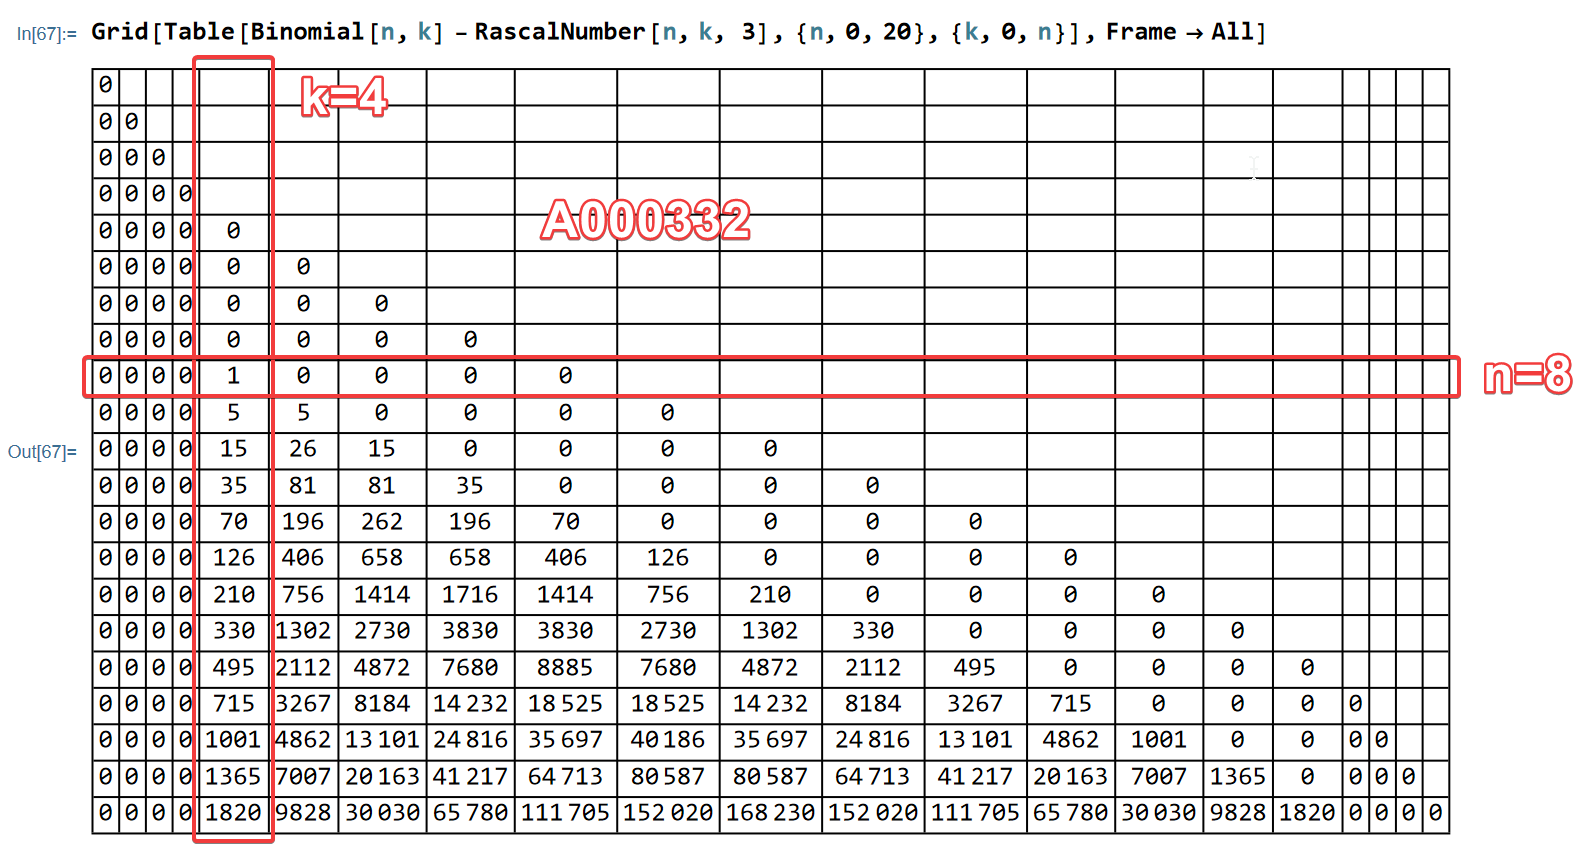
\includegraphics[width=1\textwidth]{img/01_Difference_Binomial_Rascal_i_3_BinomialCoefficients}
    ~\caption{Difference $\binom{n}{k}-\rascalNumber{n}{k}{3}$.
    Highlighted column is $\binom{n}{4}$.
    Sequence \href{https://oeis.org/A000332}{\texttt{A000332}} in the OEIS~\cite{sloane2009binomial}.}
    \label{fig:difference-binomial-rascal-i-3}
\end{figure}
We can spot that having $i=3$ the $k=4$-th column gives binomial coefficient $\binom{n}{4}$.
Indeed, this rule is true for every $i$.
\begin{proposition}
    \label{prop:row-column-difference}
    (Row-column difference.) For every fixed $i\geq0$
    \begin{align*}
        \binom{n+2i}{i} - \rascalNumber{n+2i}{i}{i-1} = \binom{n+i}{i}
    \end{align*}
    \begin{proof}
        We have previously stated that iterated rascal numbers are
        closely related to Vandermonde convolution~\eqref{eq:rascal-vandermonde-convolution}.
        Thus, proposition~\eqref{prop:row-column-difference} can be rewritten as
        \begin{align*}
            \sum_{m=0}^{i} \binom{n+i}{m} \binom{i}{i-m} - \sum_{m=0}^{i-1} \binom{n+i}{m} \binom{i}{m}
        \end{align*}
        Therefore, $\binom{n+2i}{i} - \rascalNumber{n+2i}{i}{i-1} = \binom{n+i}{i}$ is indeed true.
    \end{proof}
\end{proposition}
Proposition~\eqref{prop:row-column-difference} yields to few more identities.
Applying binomial coefficients symmetry
\begin{align*}
    \binom{n+2i}{n+i} - \rascalNumber{n+2i}{n+i}{i-1} &= \binom{n+i}{n}
\end{align*}
Taking $j=n+i$ gives
\begin{align*}
    \binom{j+i}{j} - \rascalNumber{j+i}{j}{i-1} &= \binom{j}{j-i} \\
    \binom{j+i}{i} - \rascalNumber{j+i}{i}{i-1} &= \binom{j}{i}
\end{align*}
Proposition~\eqref{prop:row-column-difference} can be generalized even further, for every fixed $i < k$.
\begin{proposition}
(Binomial coefficient difference iterated rascal number.)
    For every fixed $i < k$
    \label{prop:row-column-difference-general}
    \begin{align*}
        \binom{n}{k} - \rascalNumber{n}{k}{i} &= \sum_{m=i+1}^{k} \binom{n-k}{m} \binom{k}{k-m}
    \end{align*}
    \begin{proof}
        It is true by means of Vandermonde convolution.
    \end{proof}
\end{proposition}



    \section{Q-Binomial identities in Iterated Rascal Triangles}
    \label{sec:qbinomial-identities-in-iterated-rascal-triangles}
    Consider the table of differences of binomial coefficients and iterated rascal numbers one more time
as there is another pattern we can spot.
\begin{figure}[H]
    \centering
    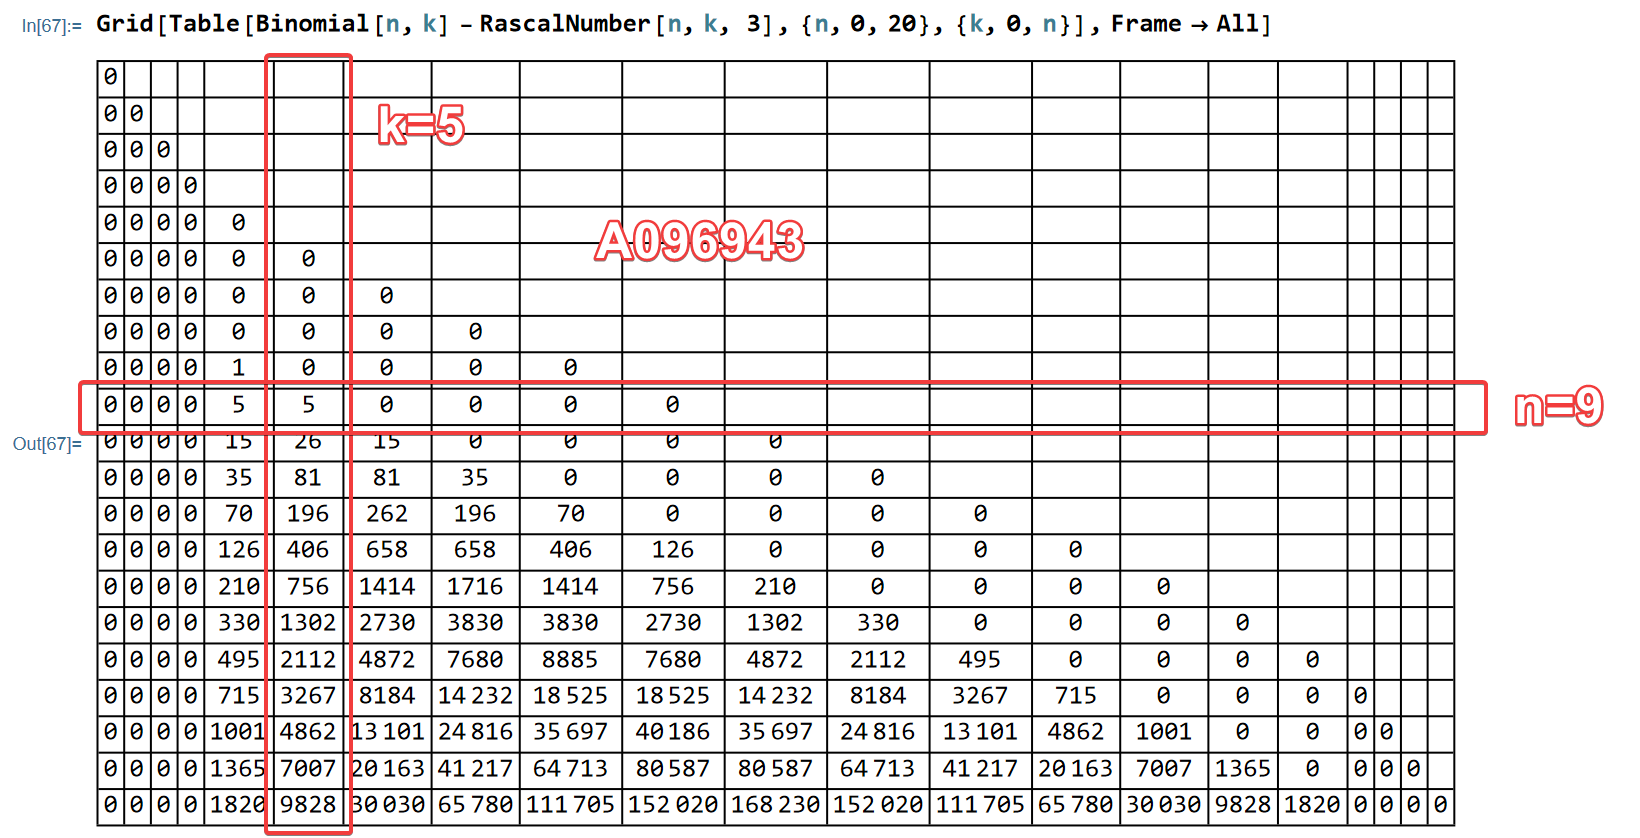
\includegraphics[width=1\textwidth]{img/03_Difference_Binomial_Rascal_i_3_OneQBinomialCoefficients}
    ~\caption{Difference $\binom{n}{k}-\rascalNumber{n}{k}{3}$.
    Highlighted column is $(1,5)$-binomial coefficient $\oneQBinomial{n}{k}{5}$.
    Sequence \href{https://oeis.org/A096943}{\texttt{A096943}} in the OEIS~\cite{sloane2004sixth}.}
    \label{fig:difference-qbinomial-rascal-i-3}
\end{figure}
The $(1,q)$-binomial coefficients $\oneQBinomial{n}{k}{q}$ are special kind of binomial coefficients defined by
\begin{definition}
    $(1,q)$-Binomial coefficient
    \begin{equation}
        \oneQBinomial{n}{k}{q} =
        \begin{cases}
            q & \mathrm{if} \; k=0, n=0 \\
            1 & \mathrm{if} \; k=0 \\
            0 & \mathrm{if} \; k > n \\
            \oneQBinomial{n-1}{k}{q} + \oneQBinomial{n-1}{k-1}{q}
        \end{cases}\label{eq:qbinomial-definition}
    \end{equation}
\end{definition}
Indeed, the relation shown in Figure~\eqref{fig:difference-qbinomial-rascal-i-3} is true for every $i$,
so that it establishes a relation between $(1,q)$-binomial coefficients and iterated rascal numbers.
\begin{proposition} (Relation between iterated rascal numbers and $(1,q)$-binomial coefficients.)
    For every $i\geq0$
    \label{prop:row-column-difference-qbinomial}
    \begin{align*}
        \binom{2i+3+j}{i+2} - \rascalNumber{2i+3+j}{i+2}{i} = \oneQBinomial{i+2+j}{i+2}{i+2}
    \end{align*}
\end{proposition}
Taking $t=i+2$ in~\eqref{prop:row-column-difference-qbinomial} yields
\begin{align*}
    \binom{2t-1+j}{t} - \rascalNumber{2t-1+j}{t}{t-2} = \oneQBinomial{t+j}{t}{t}
\end{align*}
In particular,
\begin{itemize}
    \item Having $i=1$ proposition~\eqref{prop:row-column-difference-qbinomial}
    gives the OEIS sequence \href{https://oeis.org/A006503}{\texttt{A006503}}~\cite{sloane1995n}
    such that third column of $(1,3)$-Pascal triangle
    \href{https://oeis.org/A095660}{\texttt{A095660}}~\cite{sloane2004pascal13}.
    \item Having $i=3$ proposition~\eqref{prop:row-column-difference-qbinomial}
    gives the OEIS sequence \href{https://oeis.org/A096943}{\texttt{A096943}}~\cite{sloane2004sixth}
    such that third column of $(1,5)$-Pascal triangle
    \href{https://oeis.org/A096940}{\texttt{A096940}}~\cite{sloane2004pascal}.
    \item Having $i=5$, the proposition~\eqref{prop:row-column-difference-qbinomial} yields
    the OEIS sequence \href{https://oeis.org/A097297}{\texttt{A097297}}~\cite{sloane2004seventh}
    such that seventh column of $(1,6)$-Pascal triangle
    \href{https://oeis.org/A096956}{\texttt{A096956}}~\cite{sloane2004pascal16}.
\end{itemize}



    \section{Row sums conjecture}
    \label{sec:row-sums-conjecture-for-iterated-rascal-triangles}
    In~\cite{gregory2023iterated} the authors
propose the following conjecture for row sums of iterated rascal triangles.
\begin{conj}
    \label{conjecture:row_sums}
    (Conjecture 7.5 in~\cite{gregory2023iterated}.)
    For every $i$
    \begin{align*}
        \sum_{k=0}^{4i+3} \rascalNumber{4i+3}{k}{i} &= 2^{4i+2}
    \end{align*}
\end{conj}
\begin{proof}
    Rewrite conjecture statement explicitly as
    \begin{align*}
        \sum_{k=0}^{4i+3} \sum_{m=0}^{i} \binom{4i+3-k}{m} \binom{k}{m} = 2^{4i+2}
    \end{align*}
    Rearranging sums and omitting summation bounds yields
    \begin{equation}
        \sum_{m=0}^{i}  \sum_{k} \binom{4i+3-k}{m} \binom{k}{m} = 2^{4i+2}\label{eq:row_sums_conjecture_explicit}
    \end{equation}
    In Concrete mathematics [\cite{graham1994concrete}, p.\ 169, eq (5.26)], Knuth et al.
    provide the identity for the column sum of binomial coefficients multiplication
    \begin{equation}
        \label{eq:binomial_coefficients_column_sum}
        \sum_{k=0}^{l} \binom{l-k}{m} \binom{q+k}{n} = \binom{l+q+1}{m+n+1}
    \end{equation}
    We can observe this pattern in the equation~\eqref{eq:row_sums_conjecture_explicit},
    thus the sum $\sum_{k} \binom{4i+3-k}{m} \binom{k}{m}$ equals to
    \begin{align*}
        \sum_{k} \binom{4i+3-k}{m} \binom{k}{m} = \binom{4i+4}{2m+1}
    \end{align*}
    Therefore, conjecture~\eqref{conjecture:row_sums} is equivalent to
    \begin{align*}
        \sum_{m=0}^{i} \binom{4i+4}{2m+1} = 2^{4i+2}
    \end{align*}
    Note that
    \begin{align*}
        \sum_{m=0}^{2i+1} \binom{4i+4}{2m+1} = 2^{4i+3}
    \end{align*}
    So that
    \begin{align*}
        \frac{1}{2} \sum_{m=0}^{2i+1} \binom{4i+4}{2m+1} = \sum_{m=0}^{i} \binom{4i+4}{2m+1} = 2^{4i+2}
    \end{align*}
    This completes the proof.
\end{proof}
\begin{proposition}
    For every $i$
    \begin{align*}
        \sum_{k=0}^{4i+3} \rascalNumber{4i+3}{k}{i} &= 2^{4i+2}
    \end{align*}
\end{proposition}
In particular, equation~\eqref{eq:binomial_coefficients_column_sum} assumes the following identity in
row sums of iterated rascal triangles
\begin{align*}
    \sum\limits_{k=0}^n \rascalNumber{n}{k}{i} = \sum_{m=0}^{i} \binom{n+1}{2m+1}
\end{align*}



    \section{Conclusions}\label{sec:conclusions}
    In this manuscript we have discussed new binomial identities in iterated rascal
triangles~\eqref{eq:odd-row-identity},~\eqref{prop:row-column-difference},~\eqref{prop:row-column-difference-general},
revealing a connection between the Vandermonde convolution formula and iterated rascal numbers.
We also present Vandermonde-like binomial identities~\eqref{eq:vandermonde-like-identity}.
Furthermore, we establish a relation between iterated rascal triangles
and $(1,q)$-binomial coefficients~\eqref{prop:row-column-difference-qbinomial}.
Some of the results accepted for publication in \textit{Mathematical gazette}.
Supplementary Mathematica scripts to be found at~\cite{kolosov2024identities}.



    \section{Acknowledgements}\label{sec:acknowledgements}
    Author is grateful to Oleksandr Kulkov, Markus Scheuer, Amelia Gibbs for their valuable feedback and suggestions
regarding the conjecture~\eqref{conjecture:row_sums} at MathStackExchange discussion~\cite{kolosov2024_mse_iterated}.


    \bibliographystyle{unsrt}
    \bibliography{IdentitiesInRascalTriangle}
    \noindent \textbf{Version:} \texttt{Local-0.1.0}


    \section{Addendum 1: Related OEIS sequences}\label{sec:related-oeis-sequences}
    \begin{itemize}
    \item Having $i=2$ and $k=4$: $\binom{n}{k} - \rascalNumber{n}{k}{i}$ gives
    Fifth column $(m=4)$ of $(1,4)$-Pascal triangle \url{https://oeis.org/A095667}
    \item Having $i=2$ and $k=3$: $\binom{n}{k} - \rascalNumber{n}{k}{i}$ gives
    Tetrahedral (or triangular pyramidal) numbers: $a(n) = C(n+2,3) = n*(n+1)*(n+2)/6$.
    \url{https://oeis.org/A000292}
    \item Having $i=1$ and $k=2$: $\binom{n}{k} - \rascalNumber{n}{k}{i}$ gives
    Triangular numbers: $a(n) = binomial(n+1,2) = n*(n+1)/2 = 0 + 1 + 2 + \dots + n$
    \url{https://oeis.org/A000217}
    \item Having $i=0$ and $k=3$: $\binom{n}{k} - \rascalNumber{n}{k}{i}$ gives
    Fourth column (r=3) of FS(3) staircase array.
    \url{https://oeis.org/A062748}
    \item Having $i=0$ and $k=6$: $\binom{n}{k} - \rascalNumber{n}{k}{i}$ gives
    $a(n) = binomial(n,6)-1$.
    \url{https://oeis.org/A124089}
    \item Having $i=0$ and $k=7$: $\binom{n}{k} - \rascalNumber{n}{k}{i}$ gives
    $a(n) = binomial(n,7)-1$.
    \url{https://oeis.org/A124090}
    \item Having $i=0$ and $k=2$: $\binom{n}{k} - \rascalNumber{n}{k}{i}$ gives
    $a(n) = n*(n+3)/2$.
    \url{https://oeis.org/A000096}
    \item Having $i=0$ and $k=9$: $\binom{n}{k} - \rascalNumber{n}{k}{i}$ gives
    \textit{One less than number of n-multisets chosen from a 10-set}.
    \url{https://oeis.org/A035927}
    \item Having $i=3$ and $k=4$: $\binom{n}{k} - \rascalNumber{n}{k}{i}$ gives
    Binomial coefficient $binomial(n,4) = n*(n-1)*(n-2)*(n-3)/24$.
    \url{https://oeis.org/A000332}
    \item Having $i=4$ and $k=5$: $\binom{n}{k} - \rascalNumber{n}{k}{i}$ gives
    Binomial coefficients $C(n,5)$.
    \url{https://oeis.org/A000389}
\end{itemize}



    \section{Addendum 2: Mathematica documentation}\label{sec:mathematica-documentation}
    Mathematica programs documentation.
See~\cite{kolosov2024identities}.
\begin{itemize}
    \item \texttt{ColumnIdentity1[20, 20]} validates $\rascalNumber{n}{i-k}{i} = \binom{n}{i-k}$
    \item \texttt{ColumnIdentity2[20, 20]} validates $\rascalNumber{n}{n-i+k}{i} = \binom{n}{n-i+k}$
    \item \texttt{RowIdentity1[5]} validates $\rascalNumber{2i+1-n}{k}{i} = \binom{2i+1-n}{k}$, see~\eqref{eq:odd-row-identity}
    \item \texttt{RowIdentity2[12, 5]]} validates $\rascalNumber{t-n}{k}{t-i-1}= \binom{t-n}{k}$
\end{itemize}


\end{document}
